\documentclass[conference]{IEEEtran}
\usepackage[T1]{fontenc}
\usepackage[utf8]{inputenc}
\usepackage[brazil]{babel}
\usepackage{graphicx}
\usepackage{booktabs}
\usepackage{amsmath}
\usepackage{url}

\title{Balanceamento de Carga por Eventos Discretos\\
para um Sistema Distribuído com Tráfego Bounded Pareto}

\author{\IEEEauthorblockN{Rodrigo Camargo \quad André Loubet}
\IEEEauthorblockA{RA 238257 \quad RA 253333\\
MC714, Sistemas Distribuídos, Universidade Estadual de Campinas}}

\begin{document}
\maketitle

{\footnotesize
\noindent Este trabalho implementa e avalia um balanceador de carga para três servidores. O simulador orientado a eventos discretos recebe rajadas Bounded Pareto e compara as políticas Aleatória, Round Robin e Fila Mais Curta. Cada servidor homogêneo executa até quinze requisições simultâneas, com serviço determinístico de $0{,}05$. Cada cenário usa horizonte fixo de 200 unidades e dez repetições. A análise emprega um modelo transiente de lote finito com roteamento justo. Como extensões, são avaliados servidores heterogêneos, Round Robin Ponderado, Trabalho Mínimo, Poder de Duas Escolhas, backup para estouro de buffers e uma arquitetura hierárquica de dois níveis.
\par}

\section{Introdução}
O trabalho modela uma camada de front-end distribuída que recebe uma rajada finita e encaminha cada requisição a uma réplica de serviço. Os experimentos seguem o enunciado~\cite{enunciado}: rajadas de 30, 60, 90 e 120 requisições, três servidores homogêneos, capacidade simultânea de 15 posições por servidor, serviço constante de $S=0{,}05$, horizonte $T=200$ e dez execuções independentes.

Uma rajada termina muito antes de $T$, mas o período ocioso restante pertence ao experimento. Portanto, vazão e utilização são calculadas sobre as 200 unidades, e não sobre o tempo necessário para escoar a rajada. A comparação teórica também é transiente e possui a mesma população finita, em vez de representar chegadas contínuas por tempo infinito.

\section{Arquitetura e parametrização}
\subsection{Simulador e políticas}
A implementação em Go usa uma fila mínima de eventos. Uma chegada consulta o balanceador. Havendo uma posição livre, o serviço começa e uma partida é agendada. Caso contrário, a requisição entra no buffer FIFO. Partidas precedem chegadas simultâneas. O relógio salta entre eventos, porém o resultado final avança até $T=200$, incorporando a ociosidade posterior à rajada.

Aleatória sorteia um servidor primário uniforme. Round Robin mantém um índice local à execução. Fila Mais Curta minimiza requisições ativas mais enfileiradas, com desempate pelo menor identificador. O simulador registra ocupação, fila e conclusões depois de cada evento. Geradores distintos para tráfego e roteamento asseguram o mesmo traço de chegada entre políticas em uma repetição.

\subsection{Tráfego}
A geração separa a dependência temporal da distribuição marginal. Primeiro, ruído gaussiano fracionário com $\mathcal{H}=0{,}8$ é gerado pela covariância
\begin{equation}
 \gamma_{\mathcal{H}}(k)=\frac{|k-1|^{2\mathcal{H}}-2|k|^{2\mathcal{H}}+|k+1|^{2\mathcal{H}}}{2}.
\end{equation}
Depois, a cópula gaussiana transforma cada amostra em uma Pareto Limitada em $[L,U]$, cuja densidade é
\begin{equation}
 f_X(x)=\frac{\alpha L^\alpha x^{-(\alpha+1)}}{1-(L/U)^\alpha},\quad L\leq x\leq U.
\end{equation}
Usam-se $L=0{,}0004$, $U=0{,}04$ e $\alpha=1{,}4$. Assim, $\mathcal{H}$ controla a dependência entre intervalos e $\alpha$ controla a cauda marginal. A construção de ruído fracionário segue~\cite{mandelbrot}. A Fig.~\ref{fig:traffic} confronta as amostras com a densidade teórica.

\begin{figure}[!t]
\centering
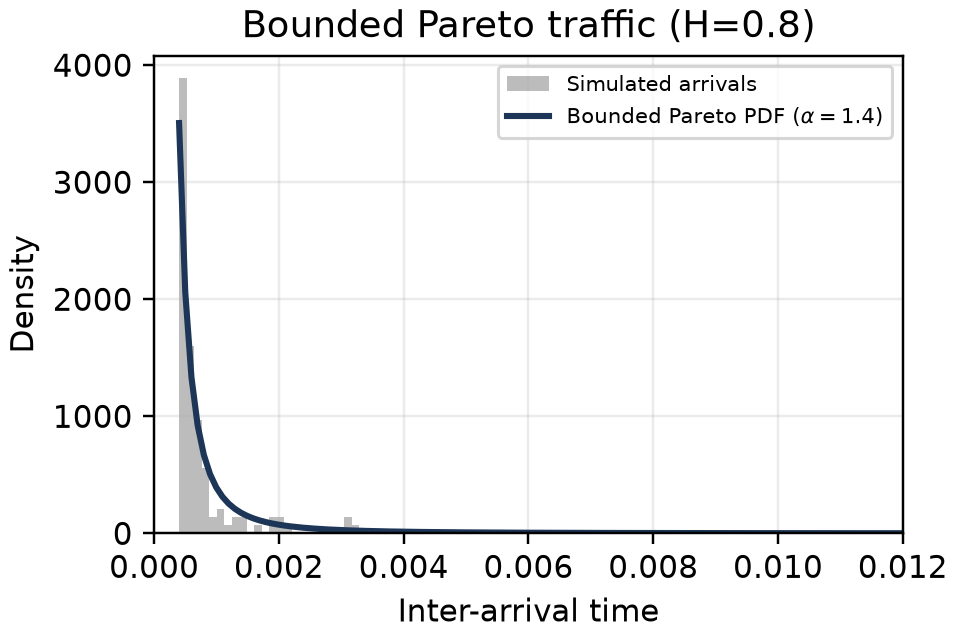
\includegraphics[width=\columnwidth]{figures/traffic_bounded_pareto.png}
\caption{Intervalos de chegada da rajada de 120 requisições e densidade Bounded Pareto.}
\label{fig:traffic}
\end{figure}

\section{Modelo analítico transiente}
Considere $m=3$ servidores e encaminhamento independente com probabilidade $p=1/m$, conforme exigido. Para uma rajada com $N$ requisições, a ocupação do servidor $s$ é
\begin{equation}
 K_s\sim\operatorname{Binomial}(N,1/m).
\end{equation}
O modelo concentra o lote em $t=0$. Condicionado a $K_s=k$, um servidor com capacidade $c_s$ e serviço $S_s$ conclui a $j$-ésima requisição no instante $S_s\lceil j/c_s\rceil$. Assim, o tempo médio esperado é
\begin{equation}
 R_0=\frac{1}{N}\sum_{s=1}^{m}\sum_{k=0}^{N}\Pr[K_s=k]
 S_s\sum_{j=1}^{k}\left\lceil\frac{j}{c_s}\right\rceil .
\end{equation}
$R_0$ é uma referência transiente de lote instantâneo. A simulação distribui chegadas em tempos positivos e, em geral, reduz sua sobreposição. O limite sem fila é a média dos $S_s$.

Como todas as requisições terminam antes de 200, vazão e utilização teóricas no horizonte são
\begin{equation}
 \Theta=\frac{N}{T},\qquad
 \rho=\frac{\sum_s E[K_s]S_s}{T\sum_s c_s}.
\end{equation}
No caso homogêneo, $\rho=NS/(3cT)$. A simulação acumula o número de posições ocupadas entre eventos e o normaliza pela capacidade total durante $T$. Essas definições medem o experimento completo. A taxa instantânea $1/E[X]$ caracteriza somente a intensidade interna da rajada e não é utilizada como vazão de longo prazo.

\section{Método experimental}
Para cada política e valor de $N$, executaram-se dez repetições com sementes reproduzíveis. A vazão é $C(T)/T$, onde $C(T)$ conta conclusões até 200. O tempo de resposta é a média entre chegada e partida das requisições concluídas. Também se mede a integral de ocupação, rejeições por buffer cheio e acionamentos do backup.
A matriz completa e os extras são reproduzidos em Linux ou Windows com Go~1.26 por \texttt{go run ./cmd/simulador}. A opção \texttt{-trace} imprime a ocupação e a fila após cada evento. As demais opções exportam resultados, repetições, tráfego e traços em CSV. O \texttt{README} fornece os comandos de compilação, testes, gráficos e PDF.

\begin{table}[!t]
\caption{Média de dez execuções. $\Theta$: req./ut. $\rho$: porcentagem. Demais colunas: resposta média.}
\label{tab:results}
\centering
\scriptsize
\begin{tabular}{rrrrrr}
\toprule
$N$ & $\Theta$ & $\rho(\%)$ & Aleat. & RR & Menor fila \\
\midrule
30  & 0,15 & 0,0167 & 0,05012 & 0,05000 & 0,05000 \\
60  & 0,30 & 0,0333 & 0,05289 & 0,05211 & 0,05212 \\
90  & 0,45 & 0,0500 & 0,05982 & 0,05753 & 0,05765 \\
120 & 0,60 & 0,0667 & 0,05810 & 0,05627 & 0,05628 \\
\bottomrule
\end{tabular}
\end{table}

\section{Resultados e discussão}
A Tabela~\ref{tab:results} e a Fig.~\ref{fig:metrics} mostram que todas as políticas concluem o lote. Por isso, a vazão é determinada por $N/200$, sem diferença entre políticas, e a utilização permanece abaixo de $0{,}067\%$. A política afeta o atraso. Em $N=120$, Round Robin reduz a resposta de $0{,}05810$ para $0{,}05627$ ($3{,}2\%$) em relação à Aleatória.

\begin{figure}[!t]
\centering

\includegraphics[width=\columnwidth]{figures/metrics_by_burst.png}
\caption{Média e desvio-padrão de dez execuções, modelo finito e referência sem fila.}
\label{fig:metrics}
\end{figure}

A Fig.~\ref{fig:model} compara o modelo diretamente à política Aleatória, cuja transição independente tem probabilidade $1/3$. A vazão analítica coincide com a simulação: $0{,}15$, $0{,}30$, $0{,}45$ e $0{,}60$. Para resposta, o lote instantâneo prevê $0{,}05015$, $0{,}06283$, $0{,}07797$ e $0{,}09439$. Os erros absolutos medidos são $0{,}00003$, $0{,}00994$, $0{,}01815$ e $0{,}03629$. A diferença cresce porque a simulação distribui chegadas em tempos positivos, enquanto o modelo concentra o lote em $t=0$. Assim, a comparação quantifica a sobreposição evitada pelo tráfego Bounded Pareto sem recorrer a Erlang-C ou regime estacionário.

\begin{figure}[!t]
\centering
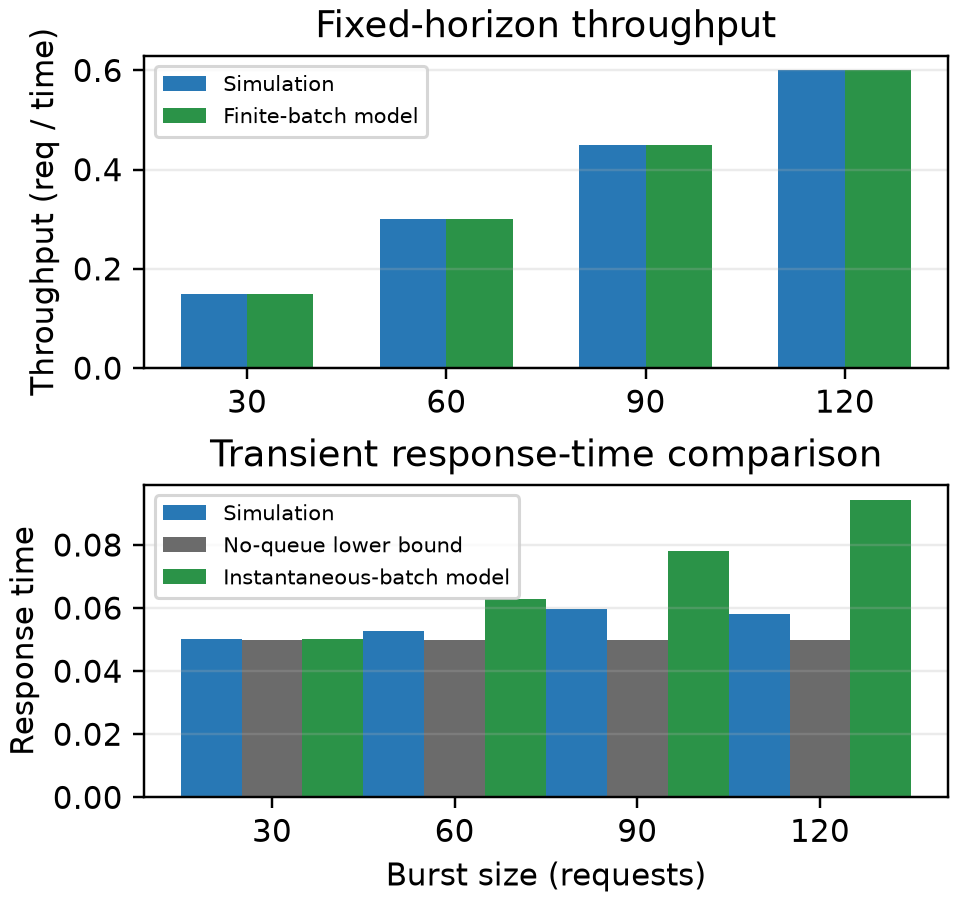
\includegraphics[width=\columnwidth]{figures/model_comparison.png}
\caption{Política Aleatória: vazão no horizonte e comparação transiente do tempo de resposta.}
\label{fig:model}
\end{figure}

\clearpage
\section{Extensões, políticas e arquiteturas adicionais}
\subsection{Servidores heterogêneos}
O primeiro extra substitui os três servidores idênticos por $(c_s,S_s)=(10,0{,}06)$, $(15,0{,}05)$ e $(20,0{,}04)$. Assim, a taxa nominal $c_s/S_s$ varia entre $166{,}7$ e $500$ requisições por unidade. Round Robin continua atribuindo um terço da carga a cada destino e, portanto, ignora essa diferença.

Foram implementadas três políticas adicionais. Round Robin Ponderado usa peso $w_s=c_s/S_s$ e o algoritmo suave. A cada decisão, soma-se $w_s$ ao acumulador de cada servidor, escolhe-se o maior acumulador e subtrai-se $\sum_s w_s$ do vencedor. Trabalho Mínimo escolhe
\begin{equation}
 s^*=\arg\min_s\frac{(a_s+q_s+1)S_s}{c_s},
\end{equation}
onde $a_s$ e $q_s$ são ocupação e fila. Poder de Duas Escolhas sorteia dois primários distintos e aplica o mesmo escore apenas ao par. A decisão compara somente dois candidatos. O simulador ainda registra todos os estados para produzir os traços exigidos.

\begin{table}[!t]
\caption{Políticas adicionais em servidores heterogêneos, $N=120$.}
\label{tab:extras}
\centering
\scriptsize
\begin{tabular}{lrrr}
\toprule
Política & $\Theta$ & Resposta & Redução vs. RR \\
\midrule
Round Robin & 0,600 & 0,06456 & 0,0\% \\
RR Ponderado & 0,600 & 0,05128 & 20,6\% \\
Trabalho Mínimo & 0,600 & 0,05101 & 21,0\% \\
Poder de Duas & 0,600 & 0,05117 & 20,7\% \\
\bottomrule
\end{tabular}
\end{table}

A Tabela~\ref{tab:extras} mostra que todas concluem 120 requisições, logo a vazão continua $0{,}60$. A diferença está no atraso. Round Robin sobrecarrega o servidor mais lento, enquanto as três políticas cientes de capacidade obtêm resposta próxima. Trabalho Mínimo apresenta a menor média, mas a vantagem de $0{,}00016$ sobre Poder de Duas é pequena diante da escala observada. Poder de Duas aproxima os dois resultados consultando somente um par.

\subsection{Buffers finitos e backup}
No segundo extra, cada primário tem buffer para duas requisições. Sem backup, a execução rejeita em média 12 requisições e produz $\Theta=0{,}540$. Um quarto servidor $(c,S)=(15,0{,}05)$ fica fora do conjunto de roteamento normal. Quando o primário selecionado não possui posição nem buffer, a requisição é desviada ao backup. Em média, ocorrem 12 acionamentos, nenhuma rejeição, $\Theta=0{,}60$ e resposta $0{,}05280$.

\begin{figure}[!t]
\centering
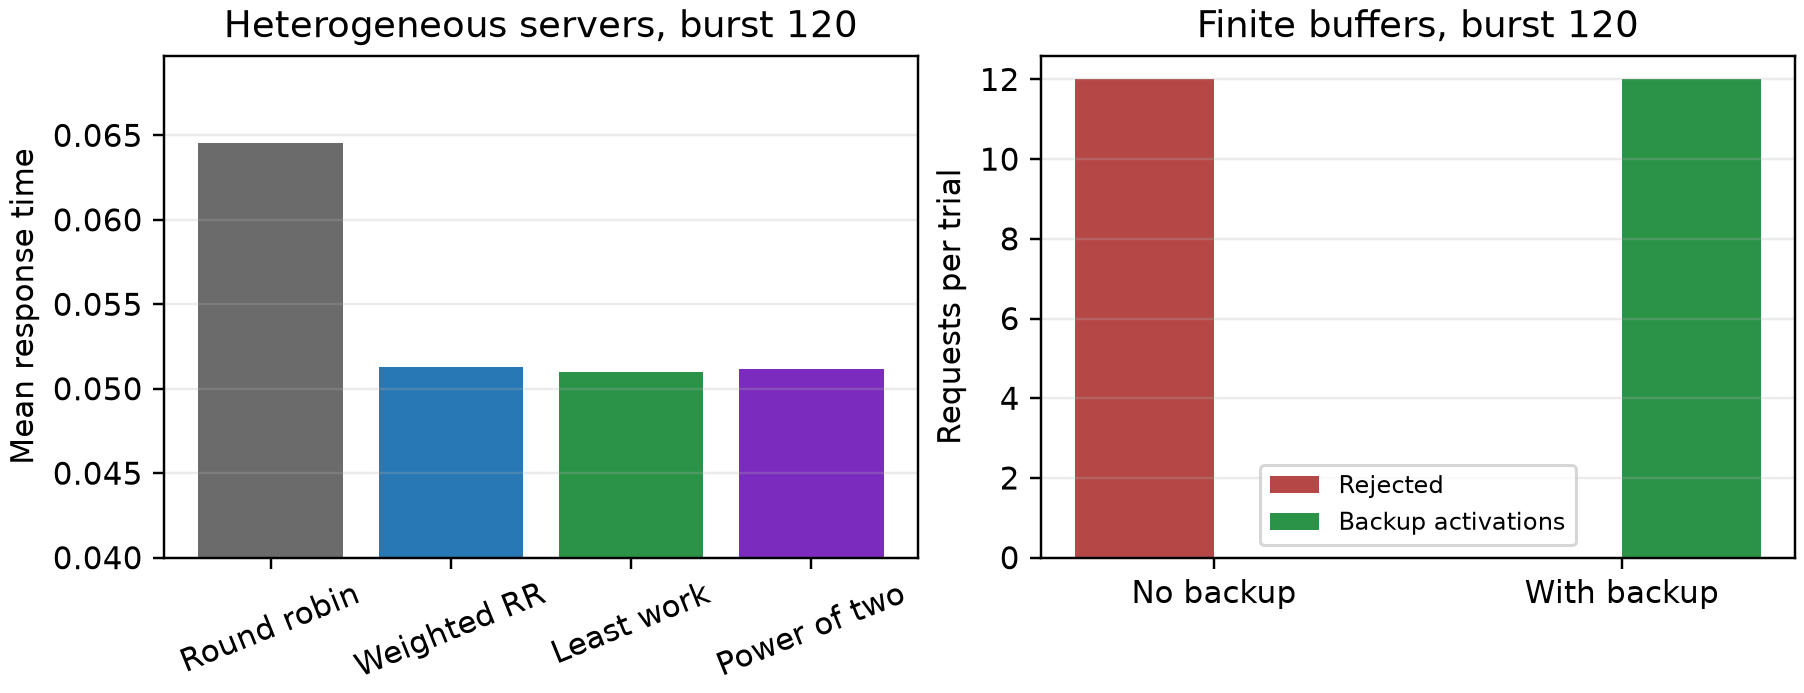
\includegraphics[width=\columnwidth]{figures/extras_comparison.png}
\caption{Políticas para servidores heterogêneos e efeito do backup com buffers finitos.}
\label{fig:extras}
\end{figure}

\subsection{Arquitetura hierárquica em dois níveis}
O terceiro extra organiza quatro servidores heterogêneos em dois pools. Um balanceador global escolhe o pool $z$ que minimiza
\begin{equation}
 G_z=\frac{1+\sum_{s\in z}(a_s+q_s)}
 {\sum_{s\in z}c_s/S_s},
\end{equation}
isto é, demanda agregada após a nova requisição dividida pela taxa nominal do pool. Em seguida, um balanceador local aplica Trabalho Mínimo somente aos dois servidores daquele pool. A separação permite que decisões locais permaneçam confinadas ao pool, enquanto o nível global troca apenas estado agregado entre grupos.

Na interpretação distribuída, o front-end é o plano de controle que toma a decisão de encaminhamento e cada servidor é uma réplica com fila privada. A medição de ocupação é uma visão local exportada ao roteador no instante da chegada. Uma implantação real enviaria essa telemetria por mensagens e poderia decidir com estado desatualizado. O simulador isola o efeito da política ao assumir leitura imediata e entrega confiável, sem somar atraso de RPC, serialização ou propagação de estado.

Como controle, a mesma topologia também executa Trabalho Mínimo plano, consultando diretamente os quatro servidores. As duas arquiteturas concluem as 120 requisições, com $\Theta=0{,}60$. A resposta é $0{,}04792$ no caso plano e $0{,}04794$ no hierárquico, diferença de apenas $0{,}00002$. Neste tráfego, não se observa penalidade relevante da hierarquia. O experimento não mede latência de rede, falhas independentes dos pools nem custo real de propagação da telemetria, portanto não implica equivalência para implantações maiores.

\begin{figure}[!t]
\centering
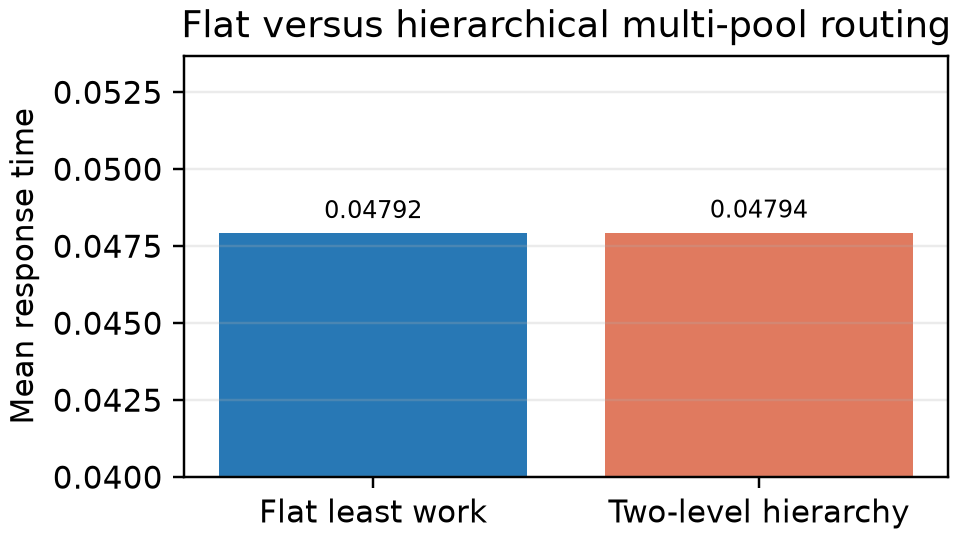
\includegraphics[width=\columnwidth]{figures/architecture_comparison.png}
\caption{Roteamento plano e hierárquico na mesma topologia de dois pools.}
\label{fig:architecture}
\end{figure}

\clearpage
\section{Validação e limitações}
A validação possui quatro níveis. Primeiro, testes determinísticos exercitam precedência de partidas, capacidade simultânea, formação de fila, término no horizonte, integral de ocupação, rejeição e ativação do backup. Segundo, testes de política verificam ciclos independentes, desempates, exclusão do backup, proporção ponderada $1{:}2{:}3$, escolha do menos carregado entre dois destinos e seleção global e local da hierarquia. Terceiro, sementes separadas garantem tráfego idêntico entre políticas. Quarto, um teste gera 2000 intervalos e confirma correlação positiva entre chegadas consecutivas para $\mathcal{H}=0{,}8$. Por fim, os CSVs são regenerados diretamente pelo executável e os gráficos apenas transformam esses dados.

O modelo analítico e a simulação não são artificialmente forçados a coincidir no tempo de resposta. O modelo concentra o lote em $t=0$ e calcula exatamente sua ocupação binomial. A simulação preserva os intervalos Bounded Pareto correlacionados. Portanto, $R_0$ é uma referência transiente de concentração, não uma previsão estacionária nem um ajuste aos dados. A igualdade de vazão decorre somente de todas as requisições terminarem antes de $T$.

O backup avaliado é recuperação de sobrecarga, não tolerância a falhas. Ele recebe uma requisição quando todos os buffers primários estão cheios. Não há detector de falhas, replicação de estado, retransmissão ou consenso. Essas escolhas delimitam o modelo a um serviço distribuído com réplicas disponíveis e deixam explícitos os mecanismos necessários para estudar indisponibilidade real.

Em uma implantação remota, a fila de cada réplica não seria memória compartilhada do front-end. Cada servidor publicaria amostras de ocupação e tamanho de fila. A decisão de Fila Mais Curta dependeria do instante de coleta, da ordem de entrega das mensagens e de atrasos de observação. A simulação representa um limite ideal no qual a amostra é atual no momento do encaminhamento. Esse limite é útil para separar o benefício da política do custo do protocolo de telemetria.

O modelo também mantém a associação entre requisição e servidor até a partida. Em um sistema distribuído, a confirmação de encaminhamento precisaria identificar a requisição de forma única para evitar duplicação após uma tentativa de reenvio. Falhas durante processamento exigiriam idempotência no serviço ou deduplicação no front-end. Esses mecanismos não alteram o escalonamento do cenário sem falhas, mas definem a diferença entre encaminhar carga e garantir execução correta diante de perdas.

A hierarquia reduz o escopo da decisão global. O controlador superior compara somente demanda agregada e taxa dos pools, enquanto o controlador local escolhe uma réplica. Essa organização reduz o volume de estado que precisa cruzar a fronteira entre pools e permite isolar políticas ou falhas por grupo. Em contrapartida, o nível global pode tomar decisões menos precisas quando sua visão agregada está atrasada. O experimento mede a consequência idealizada dessa decomposição, não o protocolo de sincronização entre controladores.

Os dez ensaios satisfazem o número pedido, mas ainda produzem incerteza visível no roteamento aleatório. Reportam-se média e desvio-padrão, sem interpretar diferenças menores que essa dispersão como vantagem conclusiva. Nos cenários de backup, utilização considera toda a capacidade provisionada, inclusive o servidor de reserva, escolha conservadora para planejamento de recursos.

\section{Conclusão}
O simulador implementa as três políticas obrigatórias, capacidade concorrente, filas finitas, monitoramento e dez repetições independentes por rajada. O horizonte fixo corrige a interpretação de vazão e utilização: as rajadas são curtas e o sistema fica ocioso na maior parte das 200 unidades. O tráfego combina a margem Bounded Pareto com dependência controlada por $\mathcal{H}=0{,}8$. O modelo binomial transiente preserva população finita, transição $1/3$ e ondas de serviço. Nos extras, políticas cientes de capacidade reduzem o atraso em aproximadamente $21\%$ nos servidores heterogêneos, o backup elimina perdas provocadas por buffers cheios e o roteamento hierárquico separa decisão global de escolha local.

\section*{Divisão de trabalho}
\textbf{Rodrigo Camargo}: projetou e implementou o simulador de eventos discretos, a fila de eventos, o gerador Bounded Pareto correlacionado, as políticas obrigatórias e adicionais, os cenários heterogêneo, de backup e hierárquico, as métricas, exportações CSV e testes automatizados. Também cuidou das sementes reproduzíveis e da execução final dos experimentos.

\textbf{André Loubet}: estruturou e revisou o relatório no formato IEEE, organizou tabelas e figuras, desenvolveu a visualização dos CSVs, confrontou resultados simulados e analíticos e revisou a apresentação das hipóteses, limitações e conclusões.

\textbf{Atividades conjuntas}: conferência dos parâmetros do enunciado, revisão do modelo transiente de lote finito, interpretação dos resultados, inspeção dos gráficos e validação do PDF e dos artefatos finais.

\begin{thebibliography}{9}
\bibitem{enunciado}
C. A. Astudillo Trujillo e D. M. da Cunha, ``Trabalho 1: Balanceador de Carga para um Sistema Distribuído,'' MC714, Unicamp, ago. 2026.
\bibitem{ross}
S. M. Ross, \textit{Introduction to Probability Models}, 12th ed. Academic Press, 2019.
\bibitem{mitzenmacher}
M. Mitzenmacher, ``The Power of Two Choices in Randomized Load Balancing,'' \textit{IEEE Transactions on Parallel and Distributed Systems}, vol. 12, no. 10, pp. 1094--1104, 2001.
\bibitem{mandelbrot}
B. B. Mandelbrot e J. W. Van Ness, ``Fractional Brownian Motions, Fractional Noises and Applications,'' \textit{SIAM Review}, vol. 10, no. 4, pp. 422--437, 1968.
\end{thebibliography}

\end{document}
